\documentclass[11pt, oneside]{report}

\usepackage{geometry}
\geometry{a4paper}
\usepackage{amsmath}
% \setmonofont[Scale=0.85]{Menlo}
\usepackage{enumitem}
\usepackage{amssymb}
\usepackage{hyperref}
\usepackage{pgfplots}
\hypersetup{linktoc=all}
\usepackage[T1]{fontenc}
\usepackage{newpxmath}
\usepackage{color}
\usepackage{mathspec}
\setmainfont [Ligatures={Common,TeX}]{Palatino Linotype} 
\usepackage{setspace}
\usepackage{wrapfig}
\usepackage{tikz}


\newcommand{\comment}[1]{\textcolor{red}{#1}}
\newcommand{\pcomment}[1]{\textcolor{green}{#1}}
\DeclareMathOperator*{\argmin}{argmin}

\linespread{1.2}

%\renewcommand{\abstractname}{Abstract}



\title{Automated Bee Pose Estimation}
\author{Jakub Nabaglo, u5558578}
\date{Semester 2, 2015}

\begin{document}
\maketitle

\begin{abstract}
    \pcomment{ABSTRACT}
\end{abstract}

\tableofcontents\newpage

\chapter{Motivation}
    Bees play a crucial role in the environment. Acting as important pollinators for numerous flowering crops, they are relied upon by our food supply and our economy, being responsible for an estimated \$200\,billion per annum in crop production[4]. Further, bees form an integral part of our ecosystems.

    Bee populations worldwide have been decreasing for decades. Research into the causes of this decline, and ways of limiting it, is crucial. It is challenged by the difficulty in tracking bee populations. That difficulty is due to a number of factors, including a lack of trained taxonomists as well as limited resources being devoted to recording bee specimens.

    A software tool capable of automatically classifying bee species from images would hence be valuable, allowing scientists and amateurs to document bee sightings by species and thus increasing the amount of data available for research. An extension of this would be a crowdsourcing application that would enable non-professionals to photograph bees that they encouter, storing the specimen species along with a geotag and a timestamp in a public database.

\chapter{Related works}
    Santana et al. (2014) have performed automated bee classification based on bee wing images labelled with the bee species and annotated with landmarks. Their process extracts wing features such as `vein length, width, curvature, angles and the area of all cells' (Santana et al, 2014, p. 253) that may be input into a generic classifier.

    \begin{wrapfigure}{l}{0.5\textwidth}
        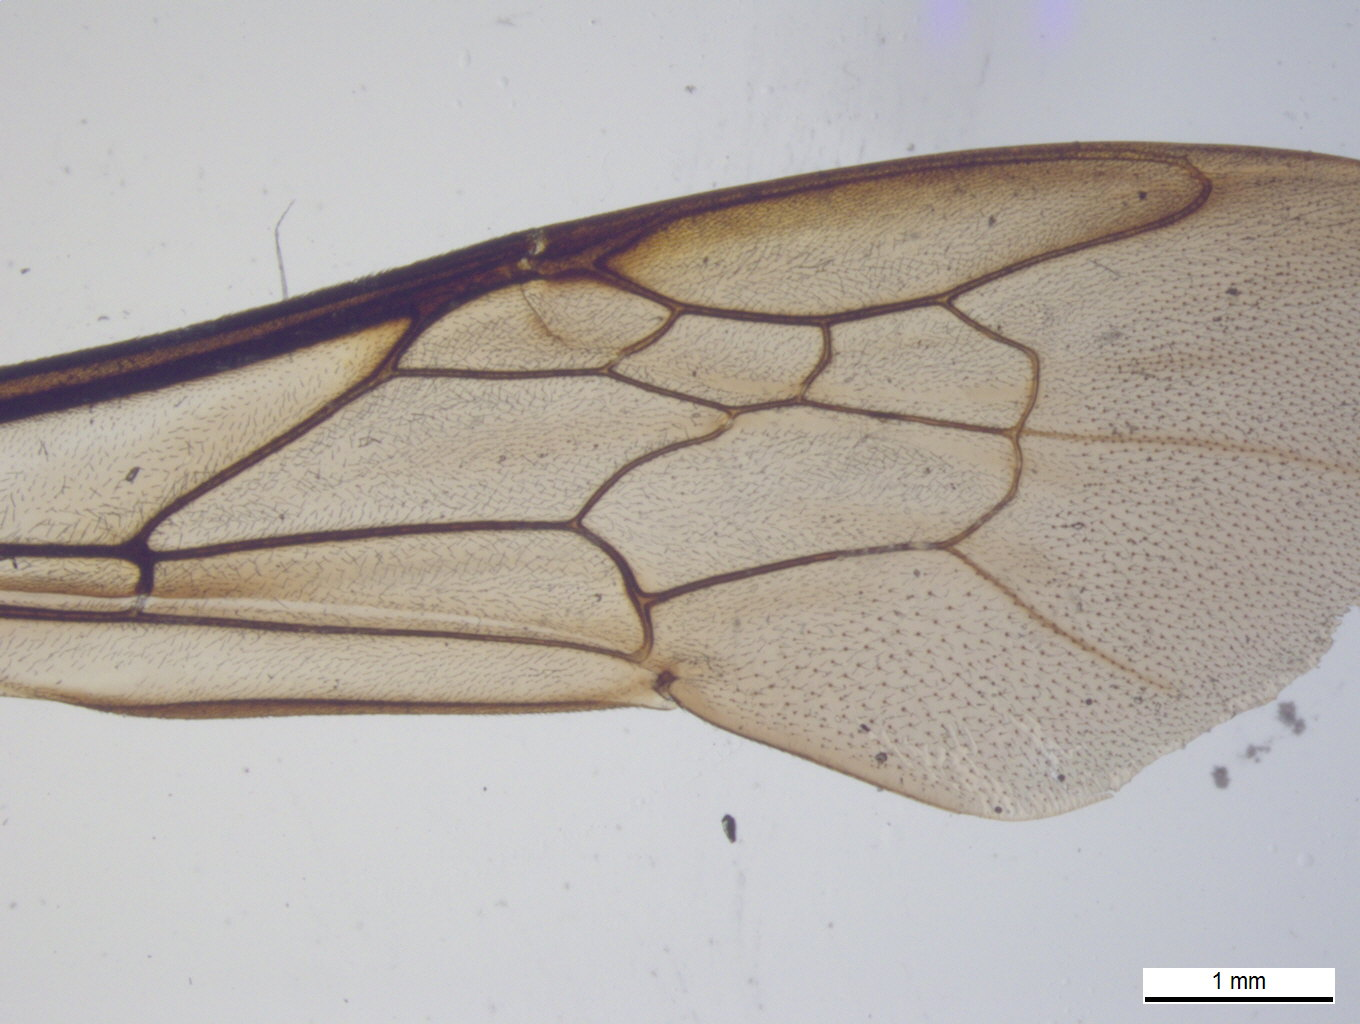
\includegraphics[width=0.5\textwidth]{santana.jpg}
        \caption{Image typical of the dataset used by Santana et al. (2014)}
        \label{fig:santana_example}
    \end{wrapfigure}

    Their approach presents several problems. In order to reliably extract features, the training and testing photographs must be captured in a highly uniform manner: the wing images must be of a high resolution and have a plain white background. An example image is shown in figure \ref{fig:santana_example}. If the goal is to enable amateurs to photograph bees and automatically classify them, the user cannot be expected to possess the equipment or motivation necessary for such consistent specimen collection.

    Further, in the work of Santana et al. (2014), images used for training and prediction must be annotated with landmarks before relevant features can be extracted. This, again, is not something an an amateur user should be expected to do.

    As such, it is necessary to develop a method to classify bees regarding of their position or orientation in the image, without requiring the user to take the photograph in a particular way, and not necessitating that they annotate landmarks. It is a logical first step to train a machine to detect the pose of the bee, as well as the bee parts useful for classification.

    Yang and Ramanan (2011) describe a model for human pose estimation. It is a supervised learning model that trains on photographs of humans that are annotated with positions of their body parts. In addition, a tree model must be defined on these parts. The tree is used in a graphical model to take advantage of relationships between body parts during training and detection.

    Although their work describes human pose estimation, it may conceivably be applied to bee pose estimation. Challenges may include the small size of some bee parts, such as antennae or legs, as well as the tendency for bee images to occlude parts: these may lower the accuracy of part detections. Large variations in bee poses may also be problematic, as this reduces the utility of the graphical model.

    \pcomment{EXPAND}

\chapter{Method}
    Experiments to perform bee pose estimation were conducted on the BEES dataset. From the BEES dataset, 250 images with all seven parts labelled were selected and split into five sets of 50. Of these, four were used for training and one was used for testing. The images in BEES deemed unsuitable for use in experiments due to bee part occlusions were used as a basis for a negative training set: bees were cropped out of these images, leaving only the background.

    The algorithm described by Yang and Ramanan (2011) was used as a basis for the experiments. A tree structure was defined on the seven bee parts labelled in BEES, with the head as the root; the antennae and the thorax as children of the head; and the wings and the abdomen as children of the thorax.

    Following training on the four training sets, predictions were made on the testing set. The testing set predictions were then displayed and visually inspected for correctness and accuracy.

\section{Algorithm}
    The algorithm used is based on the work of Yang and Ramanan (2011). It is described in more detail in their paper. A summary is provided here.

    Let $I$ be an image.

    Let $K \in\mathbb{N}$ be the number of bee parts considered, such as the head, or the wings. Then let $i \in \{1,\dots,K\}$ denote a bee part, such as the head or the left wing.

    Let $T\in\mathbb{N}$ be the number of components in the mixtures model of each part.  Let $t_i \in\{1,\dots,T\}$ be the `type' of part $i$. As an example, a bee wing can be of the folded type or of the extended type. Let $\vec{t}=(t_1,\dots,t_K)^\intercal$.

    Let $p_i=(x_i,y_i)$ be the position of part $i$ in the image $I$. Let $\vec p=(p_1,\dots,p_K)$.

    We wish to assign scores to configurations of parts. For all parts $i, j \in \{1,\dots,K\}$, let $b_i^{t_i}$ be a parameter that is greater for assignments of particular types $t_i$ to $i$. In addition, let $b_{i,j}^{t_i,t_j}$ be greater for particular co-assignments of types $t_i$ and $t_j$ to $i$ and $j$ respectively: for example, one wing being extended may make it more likely that the other wing is also extended. Define the function   \[
        S(\vec t) = \sum_{i\in V}b_i^{t_i}+\sum_{(i,j)\in E}b_{i,j}^{t_i,t_j}\textrm{,}
    \]
    where $(V,E)$ is a $K$-node relational graph, where the nodes correspond to parts and edges correspond to relation constraints between part types.

    It is now possible to define the full score for a configuration of part types $\vec t$, part positions $\vec p$ in an image $I$: \[
        S(I,\vec p, \vec t) = S(\vec t) + \sum_{i\in V}w^{t_i}_i\cdot\phi(I,p_i)
        + \sum_{(i,j) \in E}w_{i,j}^{t_i,t_j}\cdot\psi(p_i-p_j)\textrm{,}
    \]
    where $w_i^{t_i}$ and $w_{i,j}^{t_i,t_k}$ are learned parameters; where $\phi(I, p_i)$ is a HOG descriptor extracted from $p_i$ in $I$; and where $\psi(p_i-p_j)=\left((x_i-x_j)\;(x_i-x_j)^2\;(y_i-y_j)\;(y_i-y_j)^2\right)^\intercal$.

    Observing that $S(I,\vec p, \vec t)$ is linear in parameters $b_i^{t_i}$, $b_{i,j}^{t_i,t_j}$, $w_i^{t_i}$ and $w_{i,h}^{t_i,t_j}$, we can define $\vec\beta = \left(w_i^{t_i}, \dots, w_{i,h}^{t_i,t_j}, \dots, b_i^{t_i}, \dots, b_{i,j}^{t_i,t_j}, \dots\right)^\intercal$ such that $S\left(I, \vec p, \vec t\right)=\vec\beta\cdot\Phi\left(I, \vec p, \vec t\right)$ for some function $\Phi$. Learning then solves the optimisation problem: \begin{align*}
        \argmin_{w_i^{t_i}, \dots, w_{i,h}^{t_i,t_j}, \dots, \xi_i, \ldots \geq 0} &\quad\frac12\beta\cdot\beta+C\sum_n\xi_n\\
        \textrm{s.t.}\quad\forall n \in \textrm{pos} & \quad\beta\cdot\Phi(I_n, p_n, t_n) \geq 1-\xi_n \\
        \forall n \in \textrm{pos} \;\forall (p_i, t_i) & \quad\beta\cdot\Phi(I_n, p_i, t_i) \leq 1-\xi_n\textrm{.}
    \end{align*}
    The above enforces that positive examples should have scores that are greater than 1, while negative examples should score less than $-1$ for all possible part positions and types. $\xi_n$ are slack variables that penalise violations of these constraints. $C>0$ is a constant.

    Inference is then equivalent to maximising $S(I,\vec p, \vec t)$ over $\vec p$ and $\vec t$. This can be done efficiently with dynamic programming.

\section{Models for bees}
    \begin{figure}[t]
        \centering
        \begin{minipage}{0.4\textwidth}
            \centering
            \begin{tikzpicture}[scale=2.5]
                \tikzstyle{vertex}=[circle, draw=black, fill=white, line width=0.5mm, minimum size=25pt, inner sep=0pt]
                \tikzstyle{edge} = [draw, line width=1mm, -]

                \node[vertex,label=above:{Head}] (a) at (0,2) {};
                \node[vertex,label=right:{Thorax}] (b) at (0,1) {};
                \node[vertex,label=below:{Abdomen}] (c) at (0,0) {};

                \foreach \source/ \dest in {a/b, b/c}
                \path[edge] (\source) -- (\dest);
            \end{tikzpicture}
            \caption{The three-part model}
            \label{fig:3part_graph}
        \end{minipage}\hfill
        \begin{minipage}{0.55\textwidth}
            \centering
            \begin{tikzpicture}[scale=2.5]
                \tikzstyle{vertex}=[circle, draw=black, fill=white, line width=0.5mm, minimum size=25pt, inner sep=0pt]
                \tikzstyle{edge} = [draw, line width=1mm, -]

                \node[vertex,label=above:{Head}] (a) at (1,2) {};
                \node[vertex,label=right:{Thorax}] (b) at (1,1) {};
                \node[vertex,label=below:{Abdomen}] (c) at (1,0) {};
                \node[vertex,label=below:{Left wing}] (d) at (0,0) {};
                \node[vertex,label=below:{Right wing}] (e) at (2,0) {};
                \node[vertex,label=above:{Left antenna}] (f) at (0,2) {};
                \node[vertex,label=above:{Right antenna}] (h) at (2,2) {};

                \foreach \source/ \dest in {a/b, b/c, b/d, b/e, a/f, a/h}
                \path[edge] (\source) -- (\dest);
            \end{tikzpicture}
            \caption{The seven-part model}
            \label{fig:7part_graph}
        \end{minipage}
    \end{figure}
    \subsection{Three-part model}
        One of the bee part models considered is a three-part model consisting of the head, the thorax, and the abdomen, where edges running from the head to the thorax and from the thorax to the abdomen. This is illustrated in figure \ref{fig:3part_graph}.

        Since it uses only three, prominent bee parts, there are few images in the BEES dataset in which one of the parts is occluded. As such, there is a larger dataset available for training and testing.

    \subsection{Seven-part model}
        Another model considered is a seven-part model consisting of the head, the thorax, the abdomen, the left antenna, the right antenna, the left wing, and the right wing. There are edges running from the head to the thorax, from the thorax to the abdomen, as well as from the head to the antennae, and from the thorax to the wings. It is illustrated in figure \ref{fig:7part_graph}.

        Due to the higher number of parts used, it is more likely that in a particular image, a necessary part is occuded or missing. Hence, if the seven-part model is used, then the number of images available for training and testing is reduced. However, it is possible that the additional datapoints have a positive impact significant enough to compensate for a reduced training set.

\section{Evaluation}
    In our experiments, two measures were used to quantify the quality of predictions: the Probability of Correct Keypoint (PCK) and the Average Precision of Keypoints (APK). [5]

    \subsection{Probability of Correct Keypoint}
        For each image, each inferred part location is deemed either correct or incorrect. A part location is correct if it is within a threshold $\alpha\gamma$ of the ground-truth location, where $\alpha>0$ is a constant and $\gamma$ is a scaling factor equal to the distance between two particular parts in the image. The percentage of correct keypoints is then computed for each part.

    \subsection{Average Precision of Keypoints}
        Part joints can be thought of as objects to be detected. Hence, a precision-recall curve [6] can be used to evaluate this object detection accuracy. Due to this, APK penalises both false-negatives as well as false-positives.

\chapter{Results}
    \begin{itemize}
    \item
        \comment{box size comparison + graph}
    \item
        \comment{3 vs 7 part model}
    \item
        \comment{w or without augmentation}
    \item
        \comment{comparison to human performance}
    \item
        \comment{average emitting thing}
    \end{itemize}

\chapter{Future direction}
    \begin{itemize}
    \item
        \comment{use in bee classification - reference paper citing important bee parts}
    \item
        \comment{crowdsourcing}
    \end{itemize}

\chapter{References}
\pcomment{use bibtex}

[1] Y. Yang, D. Ramanan. Articulated Pose Estimation using Flexible Mixtures of Parts. CVPR 2011.

[2] http://www.stat.ucla.edu/~xianjie.chen/projects/pose\_estimation/pose\_estimation.html

[3] http://www.pcs.usp.br/~lti/joomla/index.php?option=com\_content\&view=article\&id=23\&Itemid=14

[4] Agriculture and Consumer Protection Department of the Food and Agriculture Organization of the United Nations

[5] http://www.ics.uci.edu/~dramanan/papers/pose\_pami.pdf

[6] M. Everingham, L. Van Gool, C. Williams, J. Winn, and A. Zis- serman, “The pascal visual object classes (voc) challenge,”
International Journal of Computer Vision, vol. 88, no. 2, pp. 303–
338, 2010.



\appendix
\chapter{The BEES Dataset}
    The BEES dataset was developed for this project. It is composed of 640 photographs displaying bees of various species in diverse positions.

    Each photograph in the BEES dataset displays one bee. The bee is labelled with the coordinates in the image of the middle of its head, thorax, and abdomen, as well as the tip of its right wing, left wing, right antenna and left antenna. However, in the case that one of these bee parts is occluded, no position is listed for that part. Difficult images are also tagged, and the bee is labelled with its species. Examples shown in figure \ref{fig:BEES_examples}.

\begin{figure}[h]
    \centering
    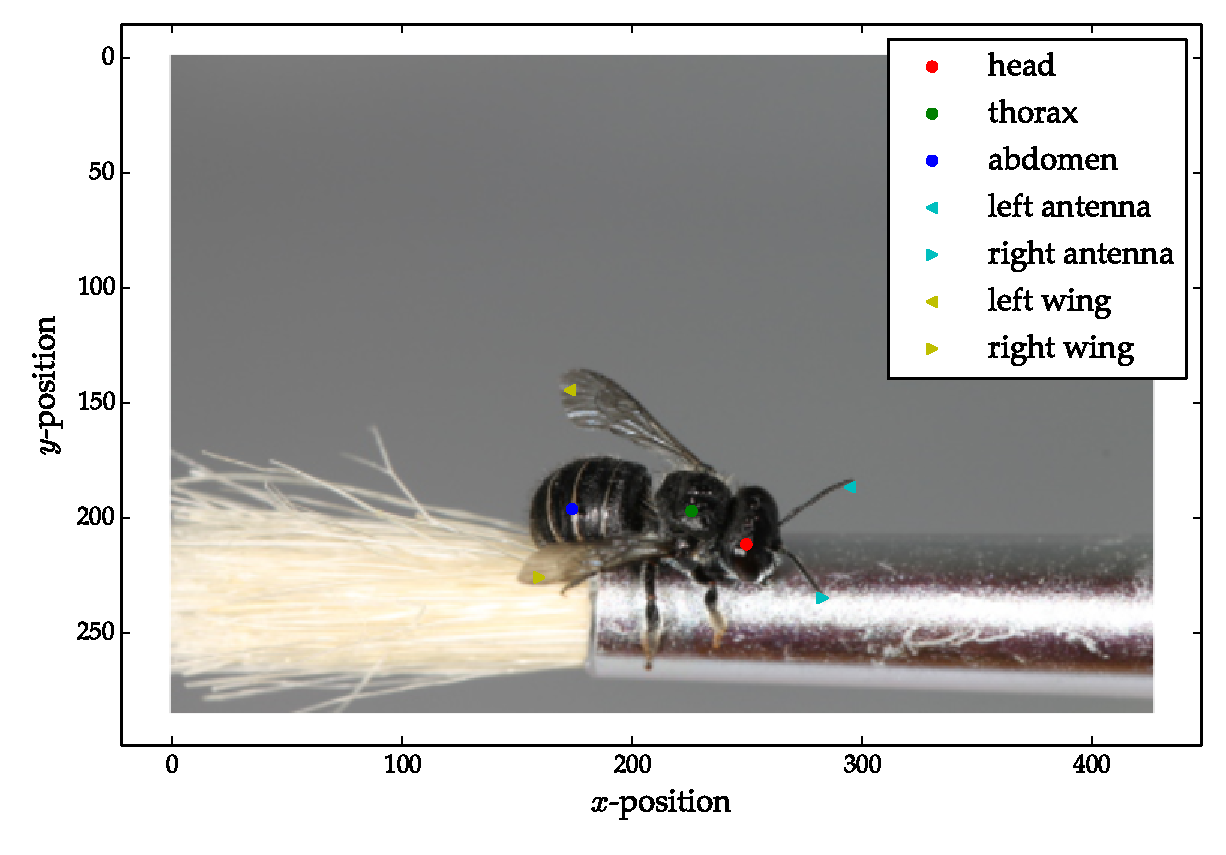
\includegraphics[width=0.424\textwidth]{b1.pdf}\hfill
    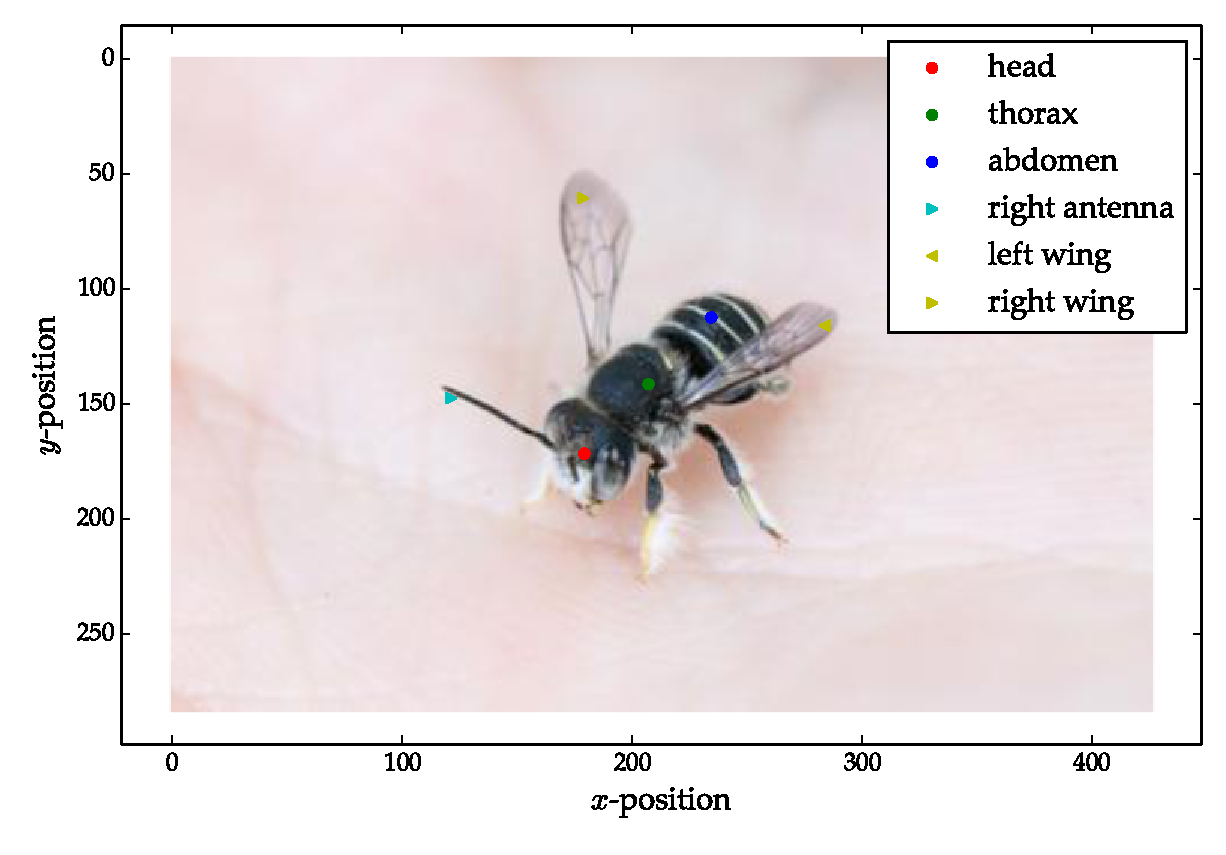
\includegraphics[width=0.424\textwidth]{b2.pdf}
    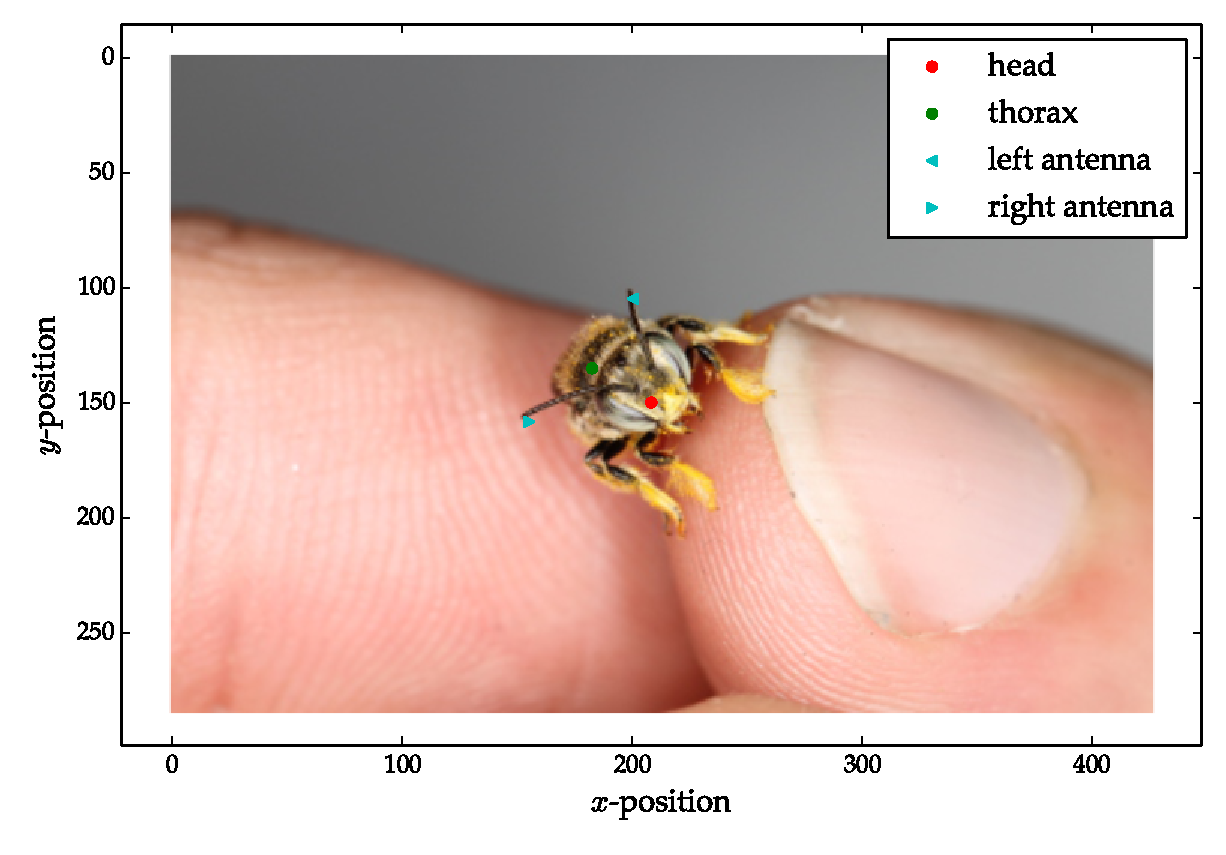
\includegraphics[width=0.424\textwidth]{b3.pdf}\hfill
    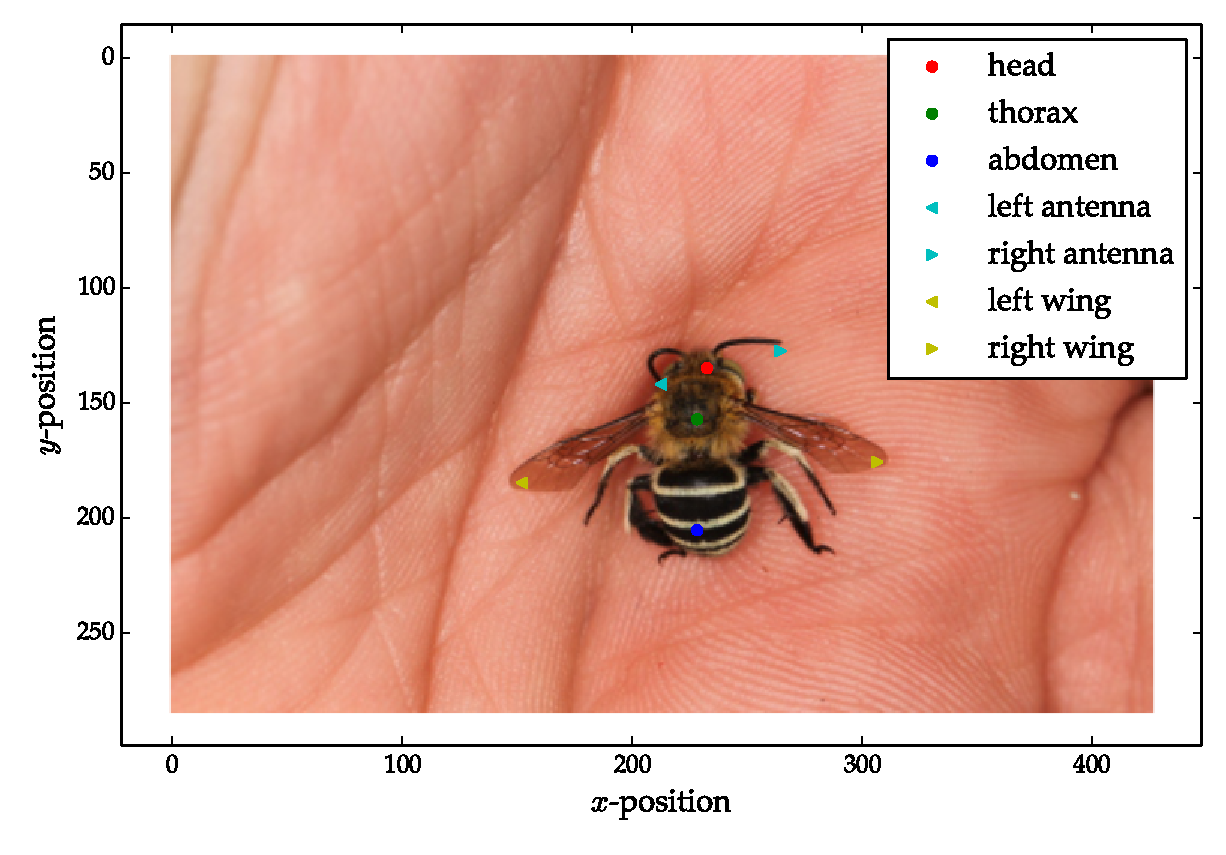
\includegraphics[width=0.424\textwidth]{b4.pdf}
    \caption{Examples of annotated images in the BEES dataset}
    \label{fig:BEES_examples}
\end{figure}

\chapter{Labelling tool}
    \comment{WRITE}
    \begin{figure}[h]
        \centering
        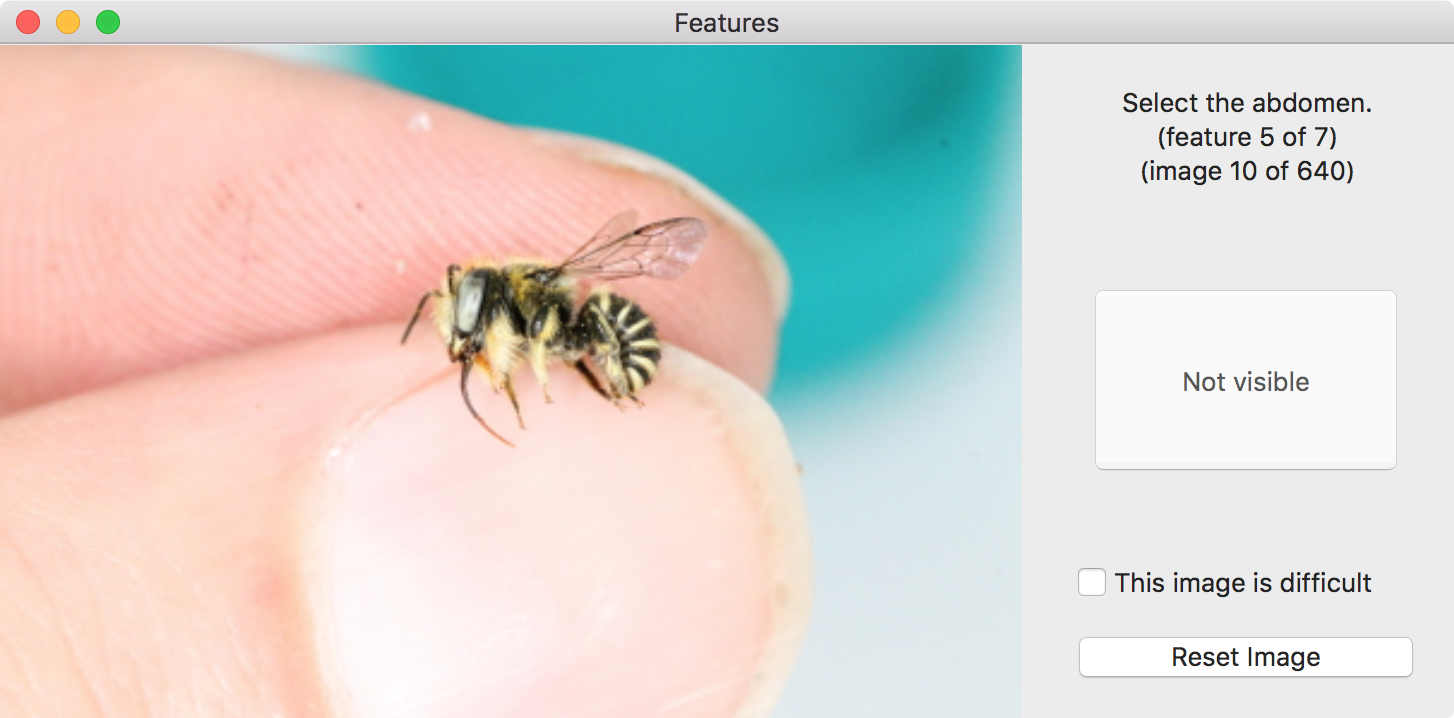
\includegraphics[width=\textwidth]{features_tool.png}\hfill
        \caption{The labelling tool}
        \label{fig:Labelling_screenshot}
    \end{figure}

\chapter{Python scripts}
    \section{Visualisation tool}
        \comment{WRITE}
        \begin{figure}[h]
            \centering
            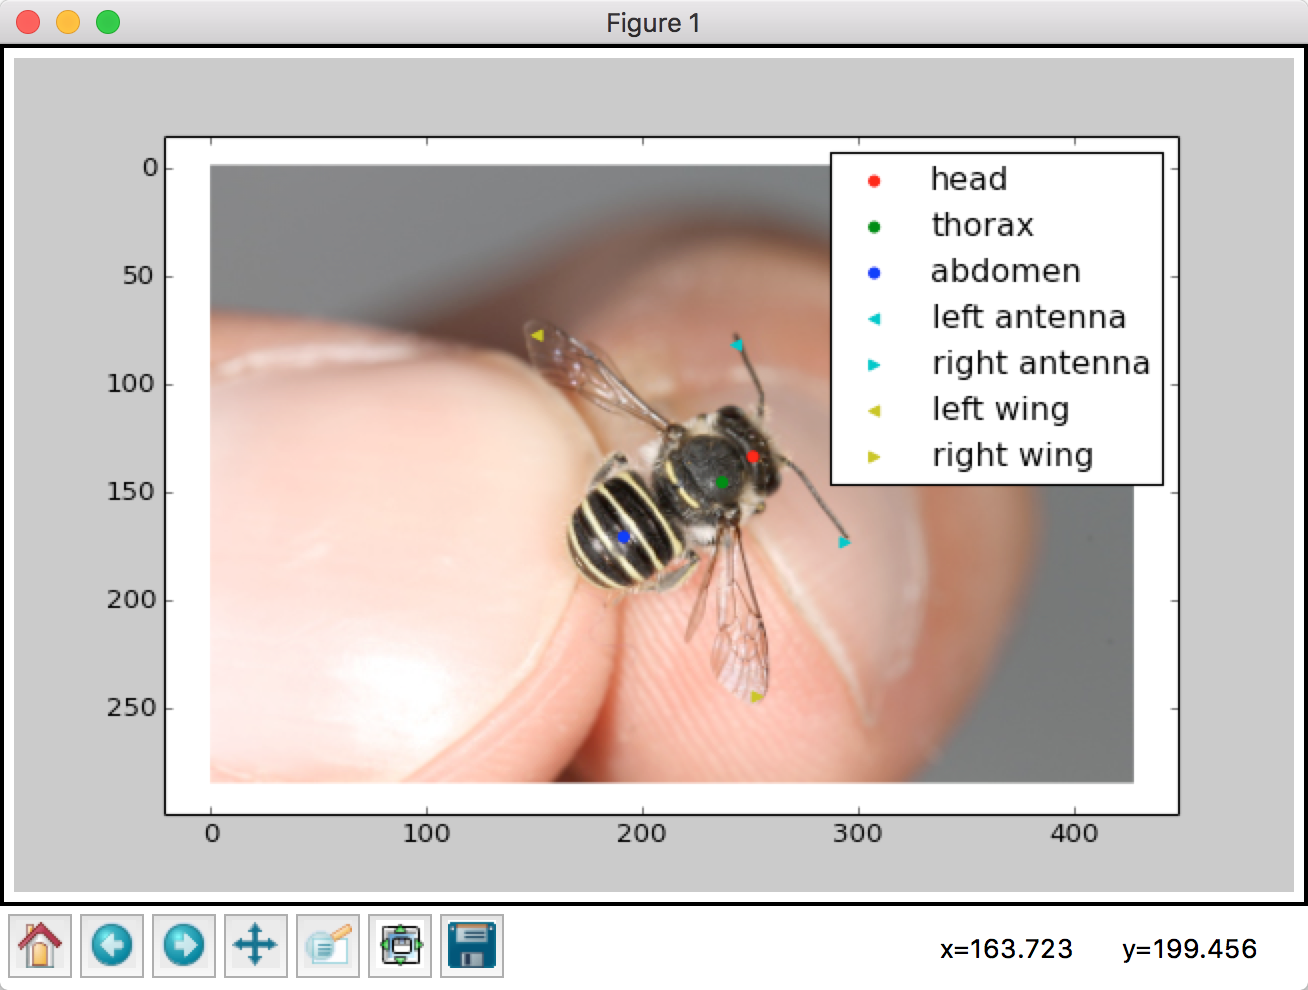
\includegraphics[width=\textwidth]{visualisation_tool.png}\hfill
            \caption{The visualisation tool}
            \label{fig:Visualisation_screenshot}
        \end{figure}

    \section{Shuffling tool}
        \comment{WRITE}
    
    \section{Conversion to .mat tool}
        \comment{WRITE}
    
    \section{Results reader}
        \comment{WRITE}

\end{document}
